%\section{intro}
The last PF candidates to be identified and reconstructed are hadrons. Hadrons are made up of quarks and gluons that are stopped by the HCAL. Some hadrons start showering in ECAL, however as seen in the previous chapter that ECAL is well calibrated for EM particles (electrons and photons), but not for hadrons.

Hadronic showers are more complicated thank EM showers because of the strong interaction with detector material. A key feature of the hadronic showers are the fluctuations in showers generated by the same incident particle. These fluctuations could be in the fraction of the energy lost (absorbed) as binding energy, particle type (pi/eta->EM showers, hadronic), particle multiplicity (secondary particles produced due to a nuclear interaction/collision). %source

To accurately reconstruct hadron (for neutral is the only way) candidates, a correction for HCAL cluster energy needs to be applied after ECAL cluster calibration. This step is important for physics analysis since as mentioned before the PF candidates will be used in reconstructing higher level physics objects.

This chapter similarly to the previous one introduced the ML method and datasets used in performing the PF HCAL cluster energy regression.

\section{GNN} %source
Graph neural network (GNN) is a type of NN that is used to process data that can be represented as graphs. Comparing to other kinds of NN, GNN can be applied on sparse data, thinly scattered data.

A graph in general consists of nodes and edges. Nodes represent the objects in our case rechits. Edges reflect the relationship between the nodes, how rechits are connected in a cluster which represent one particle.

Information in GNN can be shared between neighbors (rechits). The features’ vector of each node can be transformed into messages using dense layers which are shared between the neighbors through message passing. In this way each node learns about its neighbors and itself. (Insert here related figure %source)

\section{datasets description}
The second part of this thesis focuses on the correction of charged hadrons PF clusters for Run3. The samples used for this calibration are single Pion gun Monte Carlo (MC) samples. The datasets are centrally produced, and reconstructed under in CMSSW 12.6.4 (126X) under 23 conditions. These samples are also available through DAS web page and cover ranges of energy 2-200 GeV,200-500 GeV.

Before training the ML model, the training need to divided according to the types of hadronic showers. EH-hadrons start showering in ECAL and continue to HCAL. H-hadrons starts showering in HCAL meaning the particles do not have a nuclear interaction in ECAL. (Add figure shows EH.H location in CMS)

\section{PF cluster regression using DRN}
The ML used for charged hadron is done using a dynamic reduction network (DRN) which is based on GNN. %(Paper source , talk source).

The DRN model maps the input features onto a higher dimensional latent space and adds clustering, pooling steps to aggregate information. An overview architecture can be seen in this figure (insert here the relate figure). Summary of the steps taken during DRN training: 
step1: (Rechits) are the input for inputNet (FCNN - Fully Connected Network). 
step2: Graph Generation (KNN), EdgeConv, calculate edge weights, graph clustering (Graclus), graph pooling (add). 
Step3: Global pool (max).  
step 4: output of outputNet is (E pred, the energy reconstructed using DRN weights).

The input features used in the training are the energy (E) and (x,y,z) coordinates of individual rechits (cell, rechit are selected after dR matching). The target used for training the model is correction factor:  true energy of the generated / raw pf cluster energy that is reconstructed using detector level calibration.

Other details used for the training are:  (maybe summarize in a table, and definitions).  
the number of layers for: input 3, aggregation 2, output 2, message passing 2.  
batch size: 400. 
number of epochs trained 100. 
constant learning rate of 0.0001.  
The Loss functions used during training is defined as: (target-prediction) ^2 / target.  
The performance of the DRN training can be checked by plotting: loss vs epoch.

To test the DRN model results we calculate two quantities using the output of the DRN model (calibrated energy): energy response, energy resolution.  
Where the response = [ true energy (E true) - calibrated energy (E pre)] / E true in GeV for different true energy bins. Energy resolution = standard deviation of (E pre) / E true.  
These quantities are calculated for different regions (with different eta range): Barrel region. Endcap within the tracker region. Endcap outside the tracker region. (pt range from 1-300 GeV)

\section{results}
we present the results of response and resolution (from DRN vs Chi2) in  both Barrel region and endcap region.

\subsection{EH Hadrons}
the presented results are for the training target ratioflip
\begin{figure}
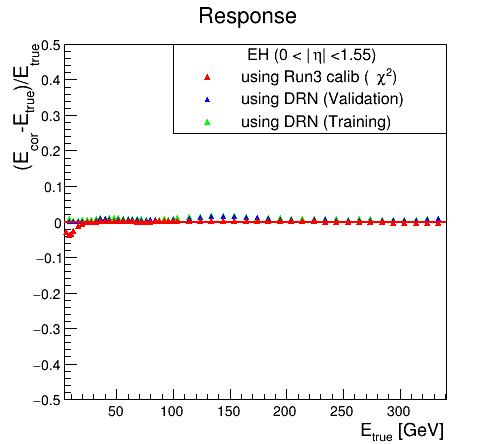
\includegraphics[width=0.495\textwidth]{./plots_pdf/HCAL_plots/Trained_target_ratioflip_0_500_10/pdf/EH_barrel/barrel_corrEtaBarrelEcalHcal.png}
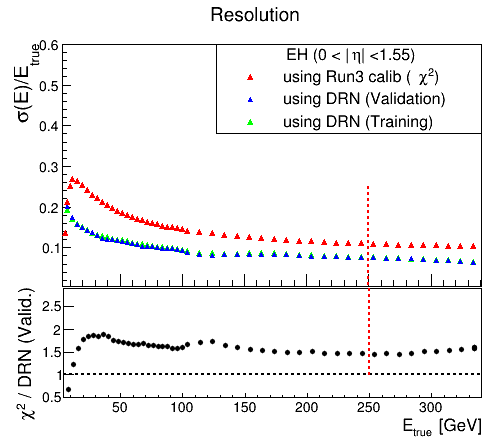
\includegraphics[width=0.495\textwidth]{./plots_pdf/HCAL_plots/Trained_target_ratioflip_0_500_10/pdf/EH_barrel/barrel_corrEtaBarrelEcalHcal_reso.png}
\caption{EH - barrel - target ratioflip}                                                                                                                                               
\end{figure}                                                                                                                                                                      

\begin{figure}                                                                                                                                                                   
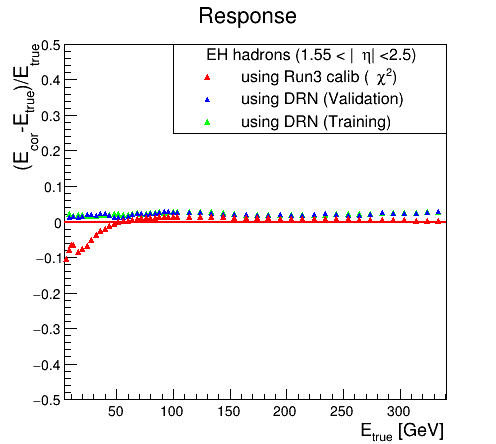
\includegraphics[width=0.495\textwidth]{./plots_pdf/HCAL_plots/Trained_target_ratioflip_0_500_10/pdf/EH_ec_in/EC_within_tracker_corrEtaEndcapEcalHcal.png}
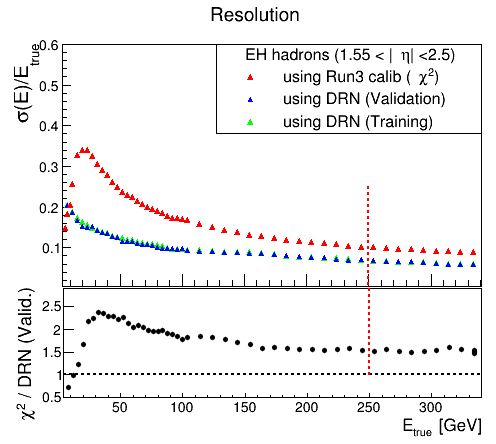
\includegraphics[width=0.495\textwidth]{./plots_pdf/HCAL_plots/Trained_target_ratioflip_0_500_10/pdf/EH_ec_in/EC_within_tracker_corrEtaEndcapEcalHcal_reso.png}
\caption{EH - endcap within tracker - target ratioflip}
\end{figure}


\begin{figure}
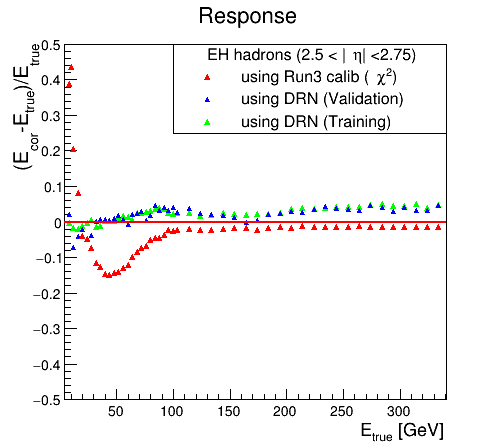
\includegraphics[width=0.495\textwidth]{./plots_pdf/HCAL_plots/Trained_target_ratioflip_0_500_10/pdf/EH_ec_out/EC_outside_tracker_corrEtaEndcapEcalHcal.png}
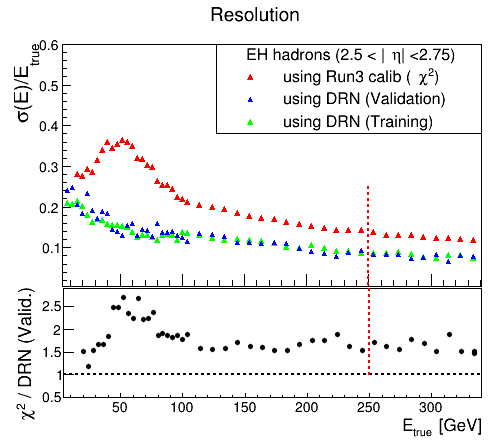
\includegraphics[width=0.495\textwidth]{./plots_pdf/HCAL_plots/Trained_target_ratioflip_0_500_10/pdf/EH_ec_out/EC_outside_tracker_corrEtaEndcapEcalHcal_reso.png}
\caption{EH - endcap outside the tracker - target ratioflip}
\end{figure}

\begin{figure}
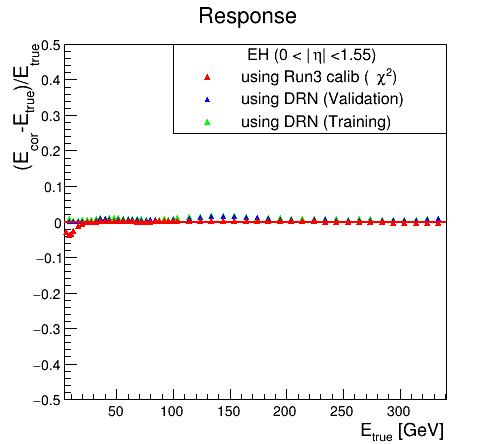
\includegraphics[width=0.495\textwidth]{./plots_pdf/HCAL_plots/Trained_target_ratioflip_0_500_10/pdf/EH_barrel/barrel_corrEtaBarrelEcalHcal.png}
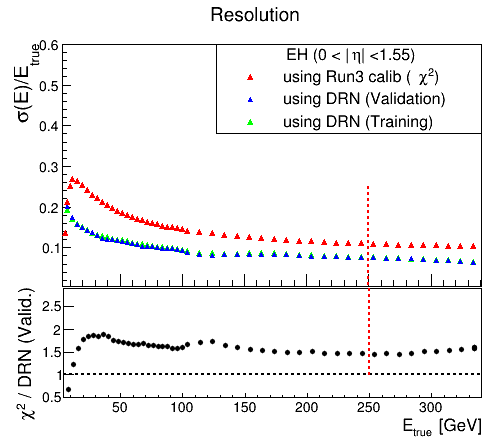
\includegraphics[width=0.495\textwidth]{./plots_pdf/HCAL_plots/Trained_target_ratioflip_0_500_10/pdf/EH_barrel/barrel_corrEtaBarrelEcalHcal_reso.png}
\caption{EH - barrel - target logratioflip}
\end{figure}

\begin{figure}
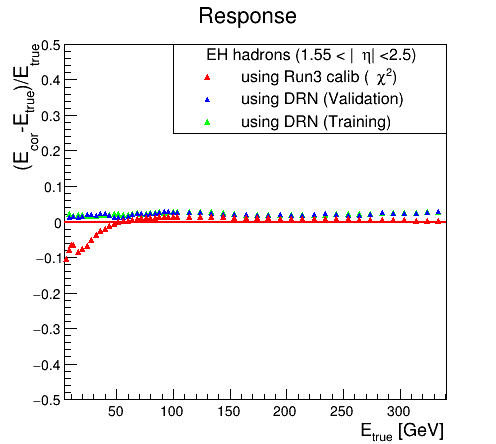
\includegraphics[width=0.495\textwidth]{./plots_pdf/HCAL_plots/Trained_target_ratioflip_0_500_10/pdf/EH_ec_in/EC_within_tracker_corrEtaEndcapEcalHcal.png}
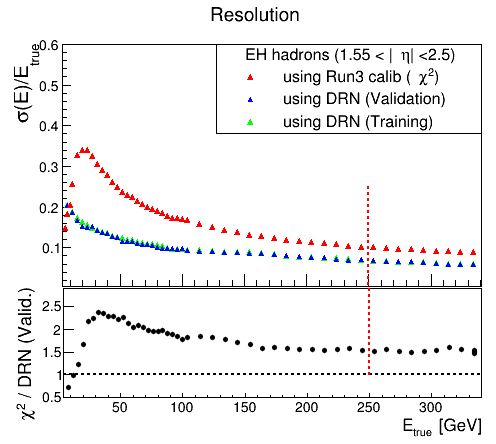
\includegraphics[width=0.495\textwidth]{./plots_pdf/HCAL_plots/Trained_target_ratioflip_0_500_10/pdf/EH_ec_in/EC_within_tracker_corrEtaEndcapEcalHcal_reso.png}
\caption{EH - endcap within tracker - target logratioflip}
\end{figure}


\begin{figure}
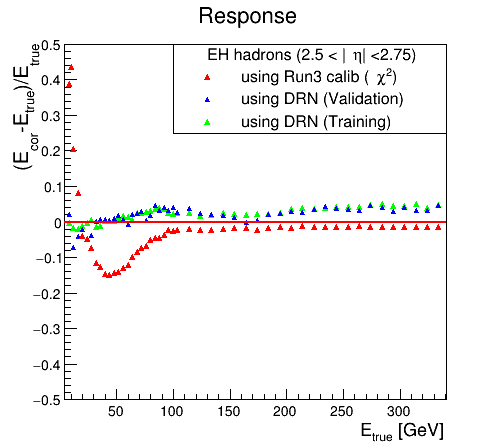
\includegraphics[width=0.495\textwidth]{./plots_pdf/HCAL_plots/Trained_target_ratioflip_0_500_10/pdf/EH_ec_out/EC_outside_tracker_corrEtaEndcapEcalHcal.png}
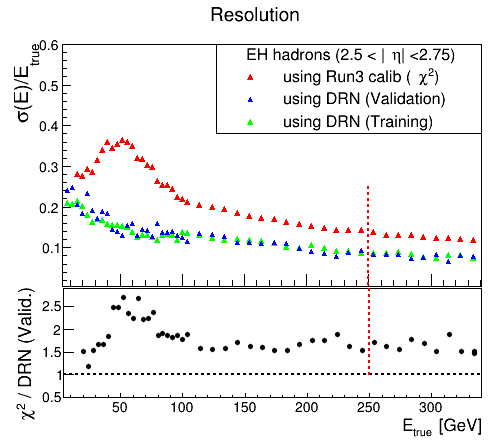
\includegraphics[width=0.495\textwidth]{./plots_pdf/HCAL_plots/Trained_target_ratioflip_0_500_10/pdf/EH_ec_out/EC_outside_tracker_corrEtaEndcapEcalHcal_reso.png}
\caption{EH - endcap outside the tracker - target logratioflip}
\end{figure}

\begin{figure}
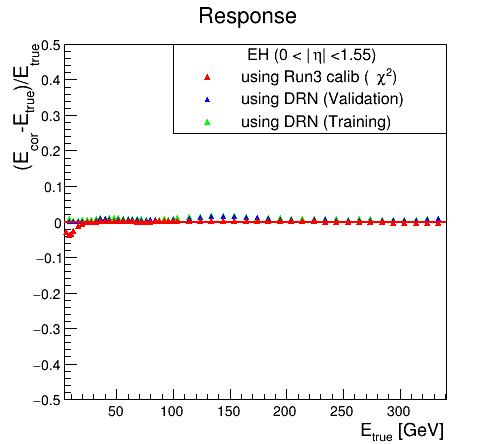
\includegraphics[width=0.495\textwidth]{./plots_pdf/HCAL_plots/Trained_target_ratioflip_0_500_10/pdf/EH_barrel/barrel_corrEtaBarrelEcalHcal.png}
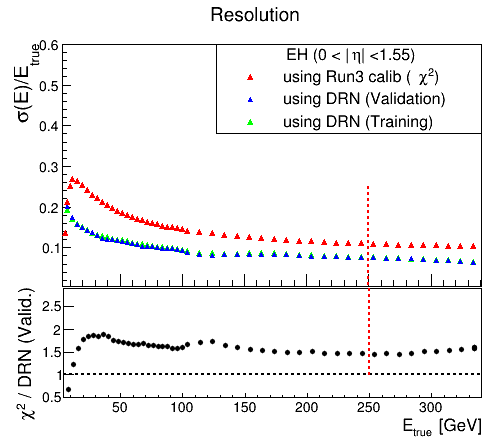
\includegraphics[width=0.495\textwidth]{./plots_pdf/HCAL_plots/Trained_target_ratioflip_0_500_10/pdf/EH_barrel/barrel_corrEtaBarrelEcalHcal_reso.png}
\caption{EH - barrel - target_ratio}                                                                                                                                               
\end{figure}                                                                                                                                                                      

\begin{figure}                                                                                                                                                                   
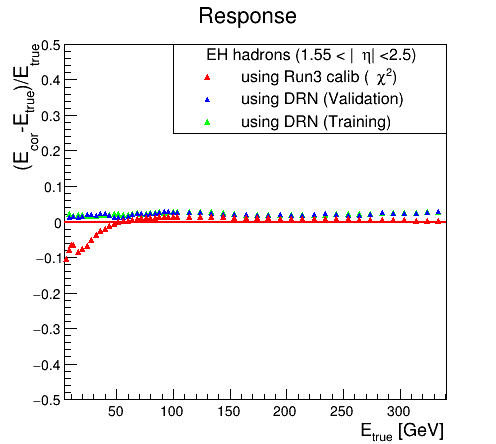
\includegraphics[width=0.495\textwidth]{./plots_pdf/HCAL_plots/Trained_target_ratioflip_0_500_10/pdf/EH_ec_in/EC_within_tracker_corrEtaEndcapEcalHcal.png}
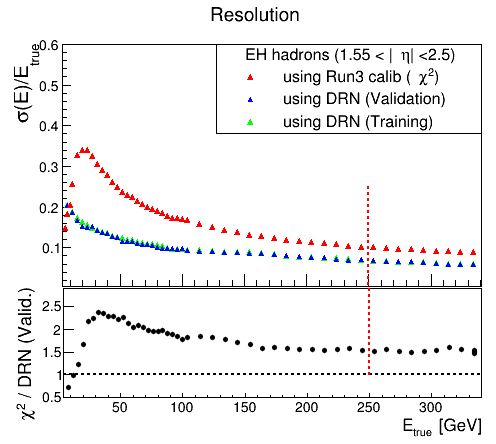
\includegraphics[width=0.495\textwidth]{./plots_pdf/HCAL_plots/Trained_target_ratioflip_0_500_10/pdf/EH_ec_in/EC_within_tracker_corrEtaEndcapEcalHcal_reso.png}
\caption{EH - endcap within tracker - target_ratio}
\end{figure}


\begin{figure}
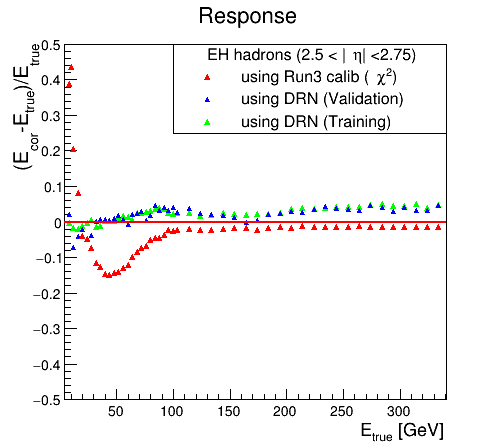
\includegraphics[width=0.495\textwidth]{./plots_pdf/HCAL_plots/Trained_target_ratioflip_0_500_10/pdf/EH_ec_out/EC_outside_tracker_corrEtaEndcapEcalHcal.png}
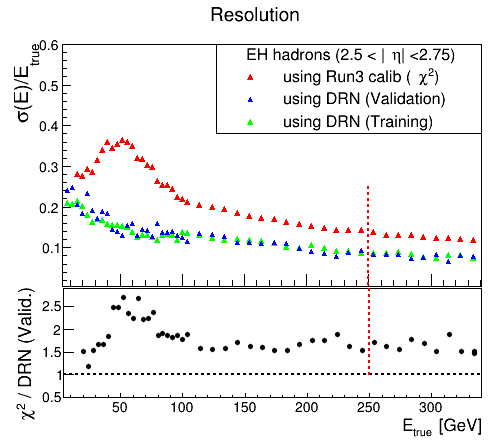
\includegraphics[width=0.495\textwidth]{./plots_pdf/HCAL_plots/Trained_target_ratioflip_0_500_10/pdf/EH_ec_out/EC_outside_tracker_corrEtaEndcapEcalHcal_reso.png}
\caption{EH - endcap outside the tracker - target_ratio}
\end{figure}

\begin{figure}
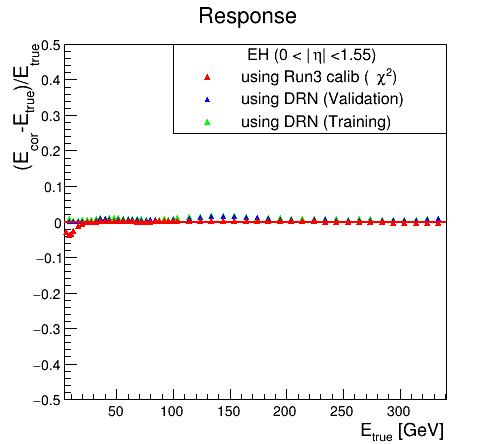
\includegraphics[width=0.495\textwidth]{./plots_pdf/HCAL_plots/Trained_target_ratioflip_0_500_10/pdf/EH_barrel/barrel_corrEtaBarrelEcalHcal.png}
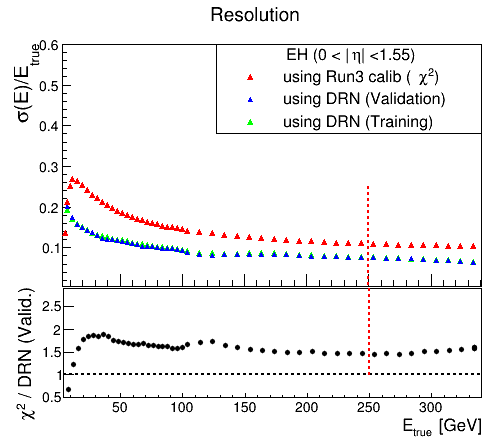
\includegraphics[width=0.495\textwidth]{./plots_pdf/HCAL_plots/Trained_target_ratioflip_0_500_10/pdf/EH_barrel/barrel_corrEtaBarrelEcalHcal_reso.png}
%\caption{EH - barrel - target trueE}
%\end{figure}

%\begin{figure}
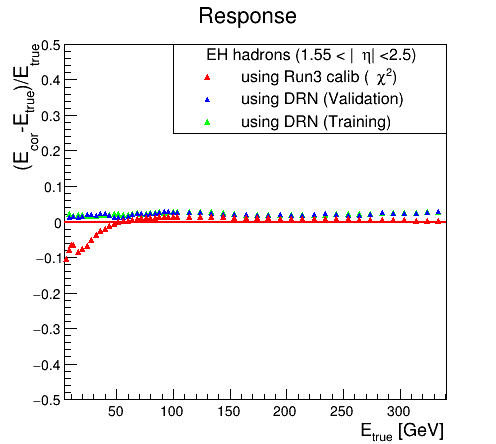
\includegraphics[width=0.495\textwidth]{./plots_pdf/HCAL_plots/Trained_target_ratioflip_0_500_10/pdf/EH_ec_in/EC_within_tracker_corrEtaEndcapEcalHcal.png}
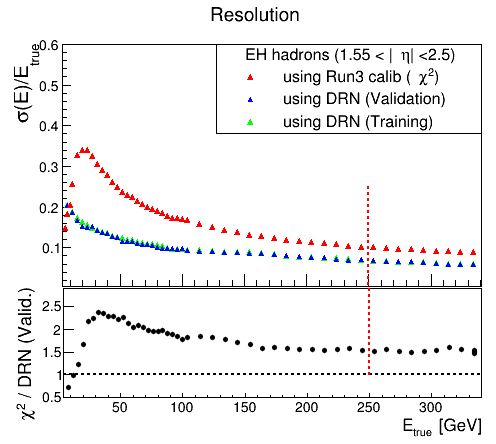
\includegraphics[width=0.495\textwidth]{./plots_pdf/HCAL_plots/Trained_target_ratioflip_0_500_10/pdf/EH_ec_in/EC_within_tracker_corrEtaEndcapEcalHcal_reso.png}
%\caption{EH - endcap within tracker - target trueE}
%\end{figure}


%\begin{figure}
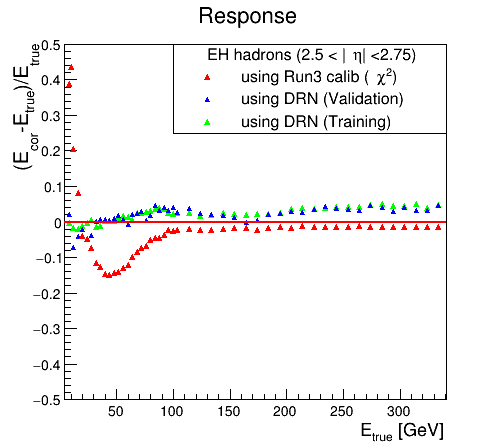
\includegraphics[width=0.495\textwidth]{./plots_pdf/HCAL_plots/Trained_target_ratioflip_0_500_10/pdf/EH_ec_out/EC_outside_tracker_corrEtaEndcapEcalHcal.png}
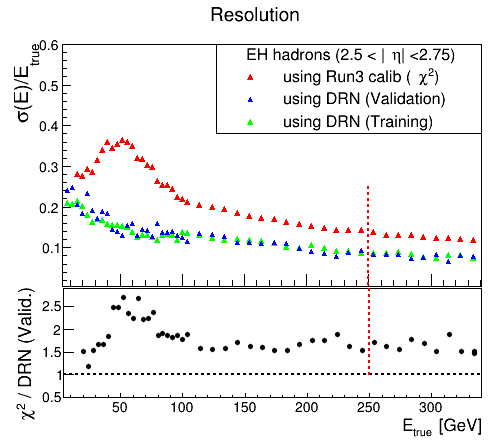
\includegraphics[width=0.495\textwidth]{./plots_pdf/HCAL_plots/Trained_target_ratioflip_0_500_10/pdf/EH_ec_out/EC_outside_tracker_corrEtaEndcapEcalHcal_reso.png}
\caption{EH - (top) barrel, (middle) endcap within tracker, (bottom) endcap outside the tracker - target trueE}
\label{fig:EH_trueE}
\end{figure}


\subsection{H hadrons}
\begin{figure}
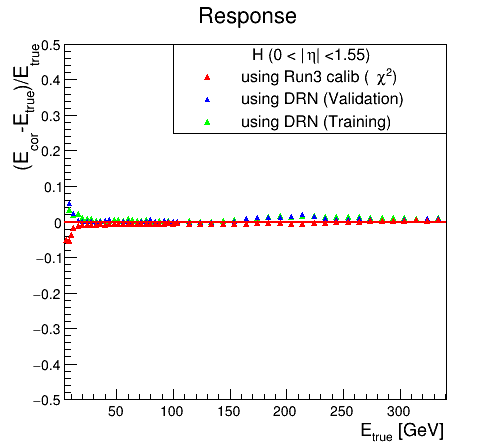
\includegraphics[width=0.495\textwidth]{./plots_pdf/HCAL_plots/Trained_target_ratioflip_0_500_10/pdf/H_barrel/barrel_corrEtaBarrelHcal.png}
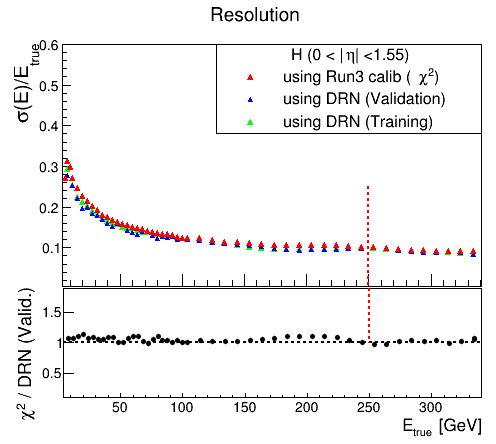
\includegraphics[width=0.495\textwidth]{./plots_pdf/HCAL_plots/Trained_target_ratioflip_0_500_10/pdf/H_barrel/barrel_corrEtaBarrelHcal_reso.png}

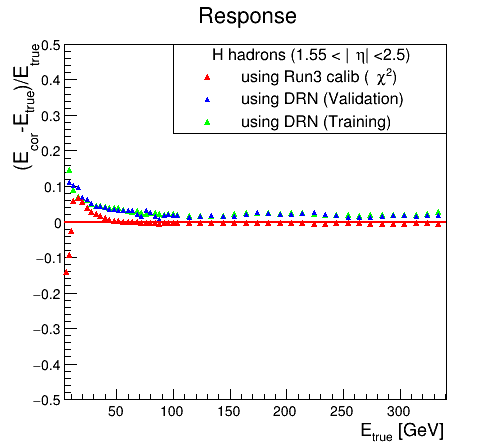
\includegraphics[width=0.495\textwidth]{./plots_pdf/HCAL_plots/Trained_target_ratioflip_0_500_10/pdf/H_ec_in/EC_within_tracker_corrEtaEndcapHcal.png}
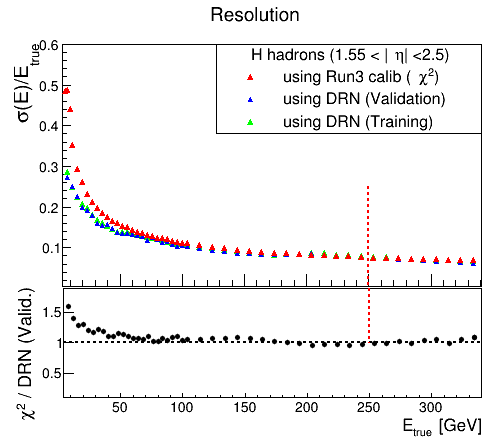
\includegraphics[width=0.495\textwidth]{./plots_pdf/HCAL_plots/Trained_target_ratioflip_0_500_10/pdf/H_ec_in/EC_within_tracker_corrEtaEndcapHcal_reso.png}

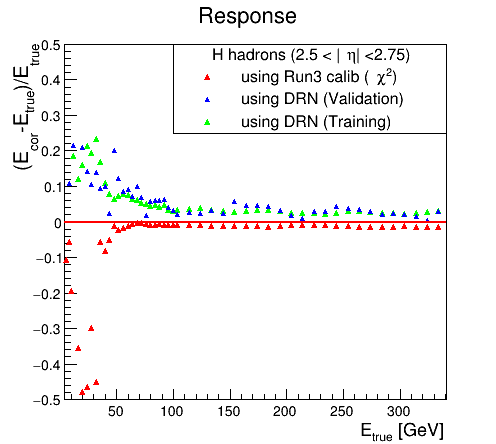
\includegraphics[width=0.495\textwidth]{./plots_pdf/HCAL_plots/Trained_target_ratioflip_0_500_10/pdf/H_ec_out/EC_outside_tracker_corrEtaEndcapHcal.png}
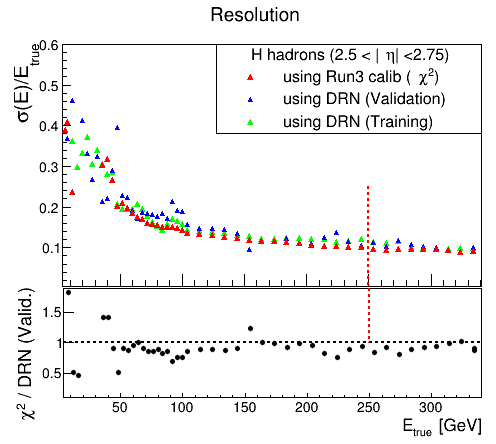
\includegraphics[width=0.495\textwidth]{./plots_pdf/HCAL_plots/Trained_target_ratioflip_0_500_10/pdf/H_ec_out/EC_outside_tracker_corrEtaEndcapHcal_reso.png}

\caption[Energy response (resolution) of the PF H-hadron cluster training traget ratioflip]{H - (top) barrel , (middle) endcap within tracker, (bottom) endcap outside the tracker - target ratioflip}
\label{fig:H_ratioflip}
\end{figure}

\begin{figure}
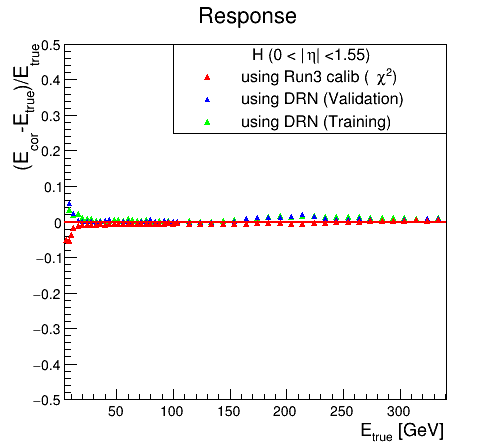
\includegraphics[width=0.495\textwidth]{./plots_pdf/HCAL_plots/Trained_target_ratioflip_0_500_10/pdf/H_barrel/barrel_corrEtaBarrelHcal.png}
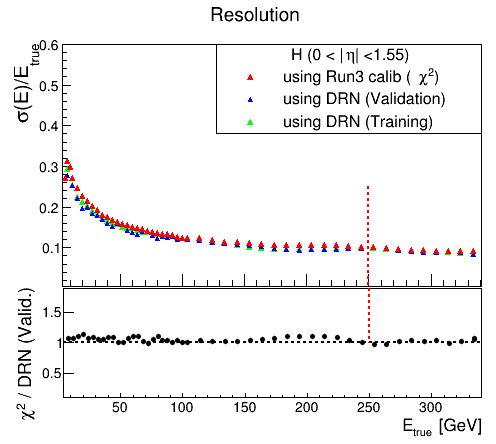
\includegraphics[width=0.495\textwidth]{./plots_pdf/HCAL_plots/Trained_target_ratioflip_0_500_10/pdf/H_barrel/barrel_corrEtaBarrelHcal_reso.png}
\caption{H - barrel - target_logratioflip}                                                                                                                                               
\end{figure}


\begin{figure}                                                                                                                                                               
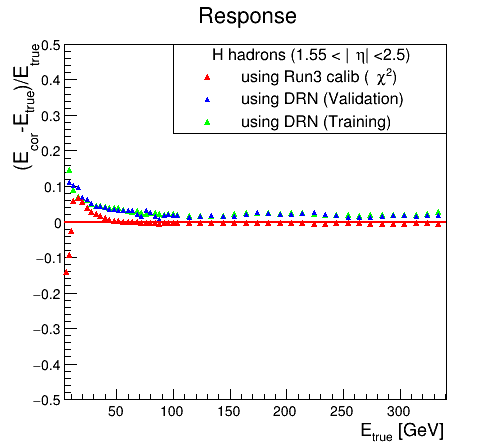
\includegraphics[width=0.495\textwidth]{./plots_pdf/HCAL_plots/Trained_target_ratioflip_0_500_10/pdf/H_ec_in/EC_within_tracker_corrEtaEndcapHcal.png}
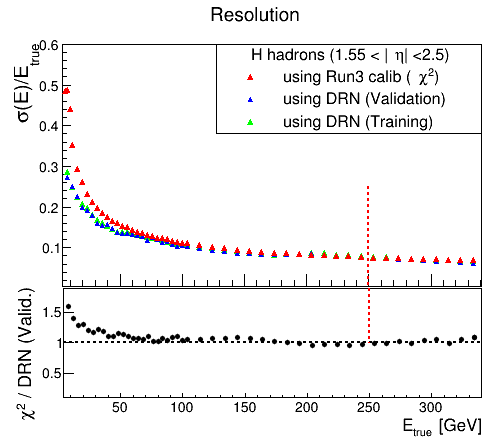
\includegraphics[width=0.495\textwidth]{./plots_pdf/HCAL_plots/Trained_target_ratioflip_0_500_10/pdf/H_ec_in/EC_within_tracker_corrEtaEndcapHcal_reso.png}
\caption{H - endcap within tracker - target_logratioflip}
\end{figure}


\begin{figure}
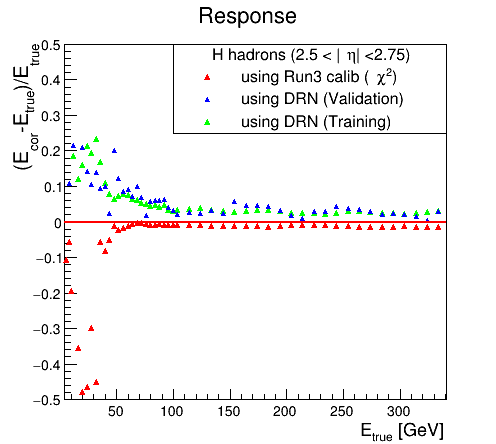
\includegraphics[width=0.495\textwidth]{./plots_pdf/HCAL_plots/Trained_target_ratioflip_0_500_10/pdf/H_ec_out/EC_outside_tracker_corrEtaEndcapHcal.png}
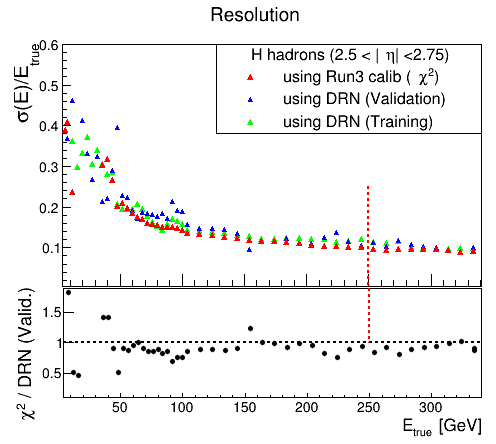
\includegraphics[width=0.495\textwidth]{./plots_pdf/HCAL_plots/Trained_target_ratioflip_0_500_10/pdf/H_ec_out/EC_outside_tracker_corrEtaEndcapHcal_reso.png}
\caption{H - endcap outside the tracker - target_logratioflip}
\end{figure}

\begin{figure}
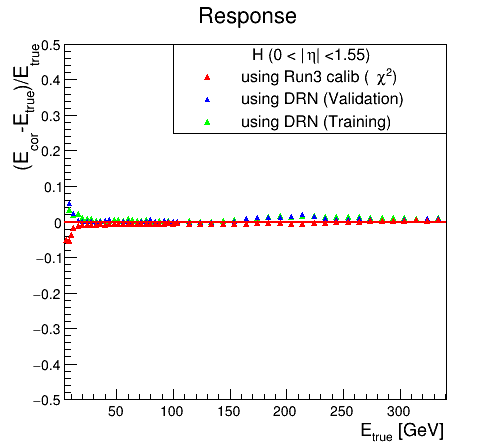
\includegraphics[width=0.495\textwidth]{./plots_pdf/HCAL_plots/Trained_target_ratioflip_0_500_10/pdf/H_barrel/barrel_corrEtaBarrelHcal.png}
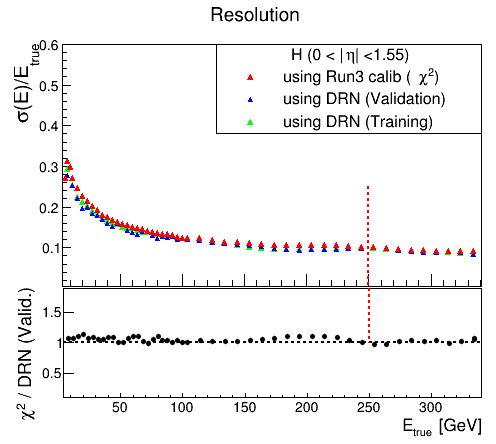
\includegraphics[width=0.495\textwidth]{./plots_pdf/HCAL_plots/Trained_target_ratioflip_0_500_10/pdf/H_barrel/barrel_corrEtaBarrelHcal_reso.png}
%\caption{H - barrel - target ratio}
%\end{figure}


%\begin{figure}
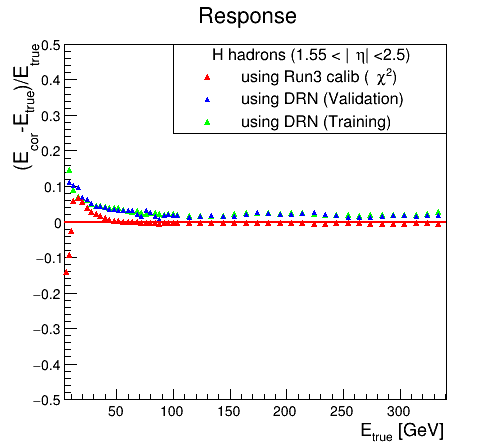
\includegraphics[width=0.495\textwidth]{./plots_pdf/HCAL_plots/Trained_target_ratioflip_0_500_10/pdf/H_ec_in/EC_within_tracker_corrEtaEndcapHcal.png}
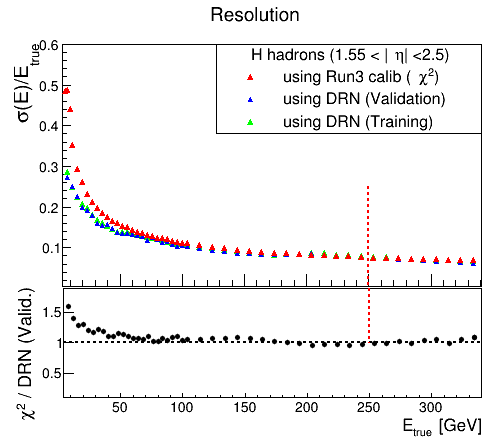
\includegraphics[width=0.495\textwidth]{./plots_pdf/HCAL_plots/Trained_target_ratioflip_0_500_10/pdf/H_ec_in/EC_within_tracker_corrEtaEndcapHcal_reso.png}
%\caption{H - endcap within tracker - target ratio}
%\end{figure}


%\begin{figure}
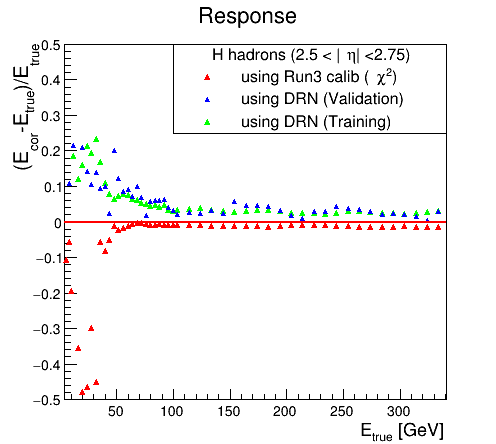
\includegraphics[width=0.495\textwidth]{./plots_pdf/HCAL_plots/Trained_target_ratioflip_0_500_10/pdf/H_ec_out/EC_outside_tracker_corrEtaEndcapHcal.png}
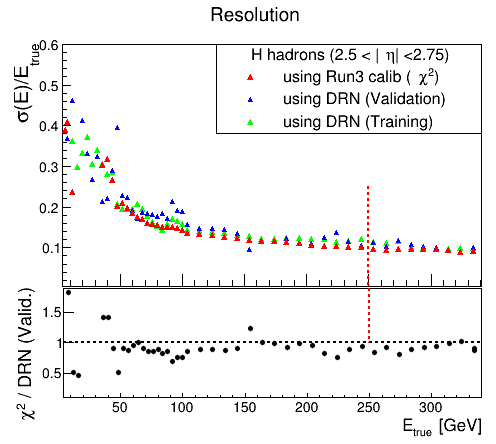
\includegraphics[width=0.495\textwidth]{./plots_pdf/HCAL_plots/Trained_target_ratioflip_0_500_10/pdf/H_ec_out/EC_outside_tracker_corrEtaEndcapHcal_reso.png}
\caption{H - (top) barrel, (middle) endcap within tracker, (bottom) endcap outside the tracker - target ratio}
\end{figure}

\begin{figure}
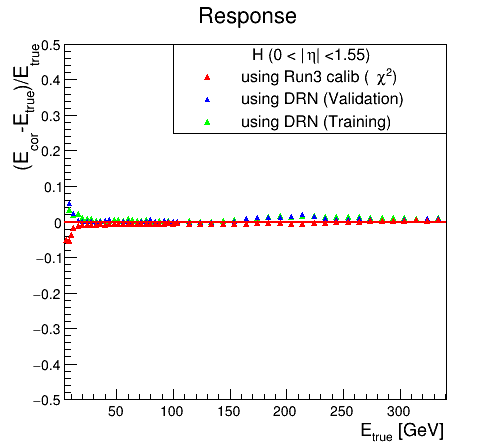
\includegraphics[width=0.495\textwidth]{./plots_pdf/HCAL_plots/Trained_target_ratioflip_0_500_10/pdf/H_barrel/barrel_corrEtaBarrelHcal.png}
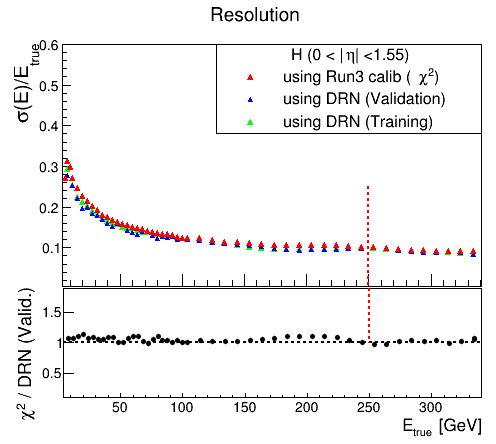
\includegraphics[width=0.495\textwidth]{./plots_pdf/HCAL_plots/Trained_target_ratioflip_0_500_10/pdf/H_barrel/barrel_corrEtaBarrelHcal_reso.png}
\caption{H - barrel - target_trueE}                                                                                                                                               
\end{figure}


\begin{figure}                                                                                                                                                               
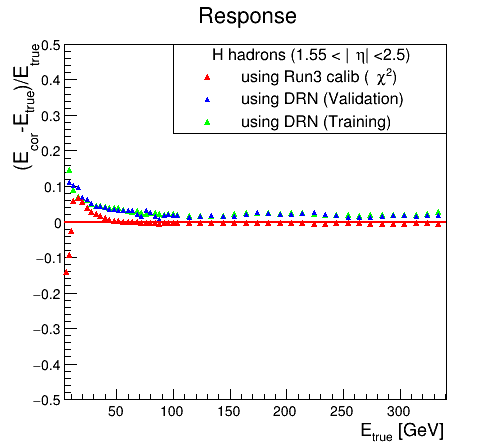
\includegraphics[width=0.495\textwidth]{./plots_pdf/HCAL_plots/Trained_target_ratioflip_0_500_10/pdf/H_ec_in/EC_within_tracker_corrEtaEndcapHcal.png}
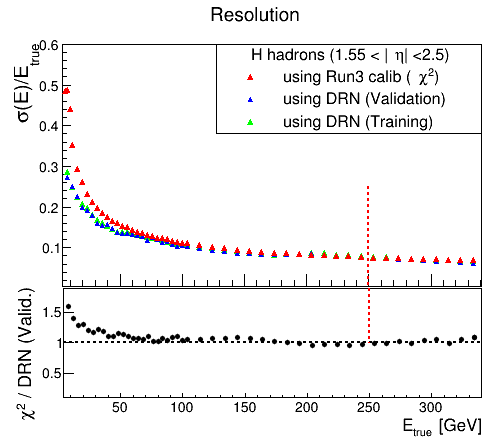
\includegraphics[width=0.495\textwidth]{./plots_pdf/HCAL_plots/Trained_target_ratioflip_0_500_10/pdf/H_ec_in/EC_within_tracker_corrEtaEndcapHcal_reso.png}
\caption{H - endcap within tracker - target_trueE}
\end{figure}


\begin{figure}
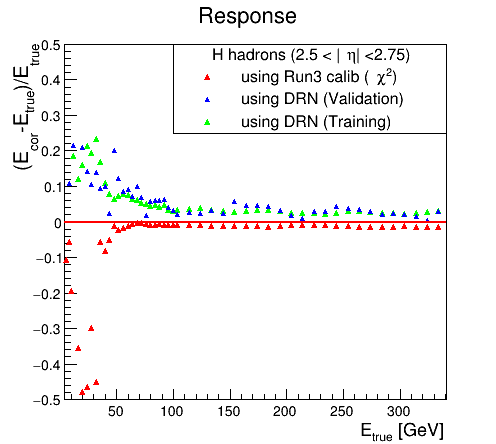
\includegraphics[width=0.495\textwidth]{./plots_pdf/HCAL_plots/Trained_target_ratioflip_0_500_10/pdf/H_ec_out/EC_outside_tracker_corrEtaEndcapHcal.png}
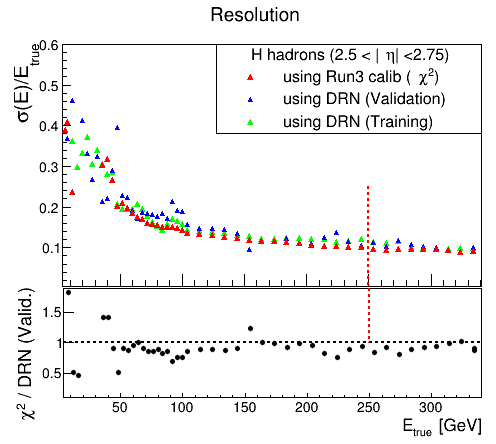
\includegraphics[width=0.495\textwidth]{./plots_pdf/HCAL_plots/Trained_target_ratioflip_0_500_10/pdf/H_ec_out/EC_outside_tracker_corrEtaEndcapHcal_reso.png}
\caption{H - endcap outside the tracker - target_trueE}
\end{figure}

